\documentclass[11pt]{article}
\usepackage{classTools}
\usepackage{graphicx}
\def\draft{1}

\begin{document}
\psHeader{0}{Wed 2023-09-13 (11:59PM)}

The purpose of this problem set is to reactivate your skills in proofs and programming from CS20 and CS32/CS50. For those of you who haven't taken one or both those courses, the problem set can also help you assess whether you have acquired sufficient skills to enter CS120 in other ways and can fill in any missing gaps through self-study. Even for students with all of the recommended background, this problem set may still require a significant amount of thought and effort, so do not be discouraged if that is the case and do take advantage of the staff support in section and office hours. 

For those of you who are wondering whether you should wait and take CS20 before taking CS120, we encourage you to also complete  \href{https://drive.google.com/file/d/1QIJR6sb9hfkK67PhpQaK9KQBzYwzXvsW/view}{the CS20 Placement Self-Assessment}.  Some problems there that are of particular relevance to CS120 and are complementary to what is covered below are Problems 2 (counting), 4 (comparing growth rates), 9 (quantificational logic), and 12 (graph theory). 

Written answers must be submitted in pdf format on Gradescope. Although \LaTeX{} is not required, it is strongly encouraged. You may handwrite solutions so long as they are fully legible. The \texttt{ps0} directory, which contains your code for problems 1a and 1c, must be submitted separately to an autograder on Gradescope. Be sure to pull the starter code from the \href{https://github.com/Harvard-CS-120/cs120}{cs120 GitHub repository}.

 \newcommand{\children}{\mathit{children}}
 \newcommand{\parent}{\mathit{parent}}
 
\begin{enumerate}
\item (Binary Trees) 
 In the \href{https://github.com/Harvard-CS-120/cs120}{cs120 GitHub repository}, we have given you a Python implementation of a binary tree data structure, as well as a collection of test trees built using this data structure.  We specify a binary tree by giving a pointer to its {\em root}, which is a special {\em vertex} (a.k.a. {\em node}), and giving every vertex pointers to its {\em children} vertices and its {\em parent} vertex as well as an identifying {\em key}: 
 
 \begin{verbatim}
    class BinaryTree:
        def __init__(self, root):
            self.root: BTvertex = root
 
    class BTvertex:
        def __init__(self, key):
            self.parent: BTvertex = None
            self.left: BTvertex = None
            self.right: BTvertex = None
            self.key: int = key
            self.size: int = None
 \end{verbatim}


 In CS50, the concept of a Python \texttt{class} was not covered. Here, with \texttt{BinaryTree} and \texttt{BTvertex}, we are using them in the same way as a \texttt{struct} in C. An object \btv\ of the \texttt{BTvertex} class contains five attributes, which we list with the type of the object we expect to be named by each attribute (using the Python type annotation syntax). These attributes can be accessed as \texttt{v.parent}, \texttt{v.left}, \texttt{v.right}, \texttt{v.key}, and \texttt{v.size}. 
 For example, \texttt{v.left.key} is the key associated with \btv's left child. An object of the \texttt{BinaryTree} class contains only one attribute, which is the \texttt{BTvertex} object that is the root of our binary tree. You can create a \texttt{BinaryTree} object as follows:
 
\begin{verbatim}
root = BTvertex(120)
tree = BinaryTree(root)
tree.root.left = BTvertex(121)
tree.root.right = BTvertex(124)
\end{verbatim}

You can then print attributes of the newly created \texttt{BinaryTree} object:
\begin{verbatim}
print(tree.root.key)
>> 120
print(tree.root.left.key)
>> 121
\end{verbatim}
 

 Classes are more general than structs because they can also have private attributes and methods that operate on the attributes, allowing for object-oriented programming. However, you won't need that generality in this problem set.

 Here is an instance \treeT\ of \texttt{BinaryTree}:
 
 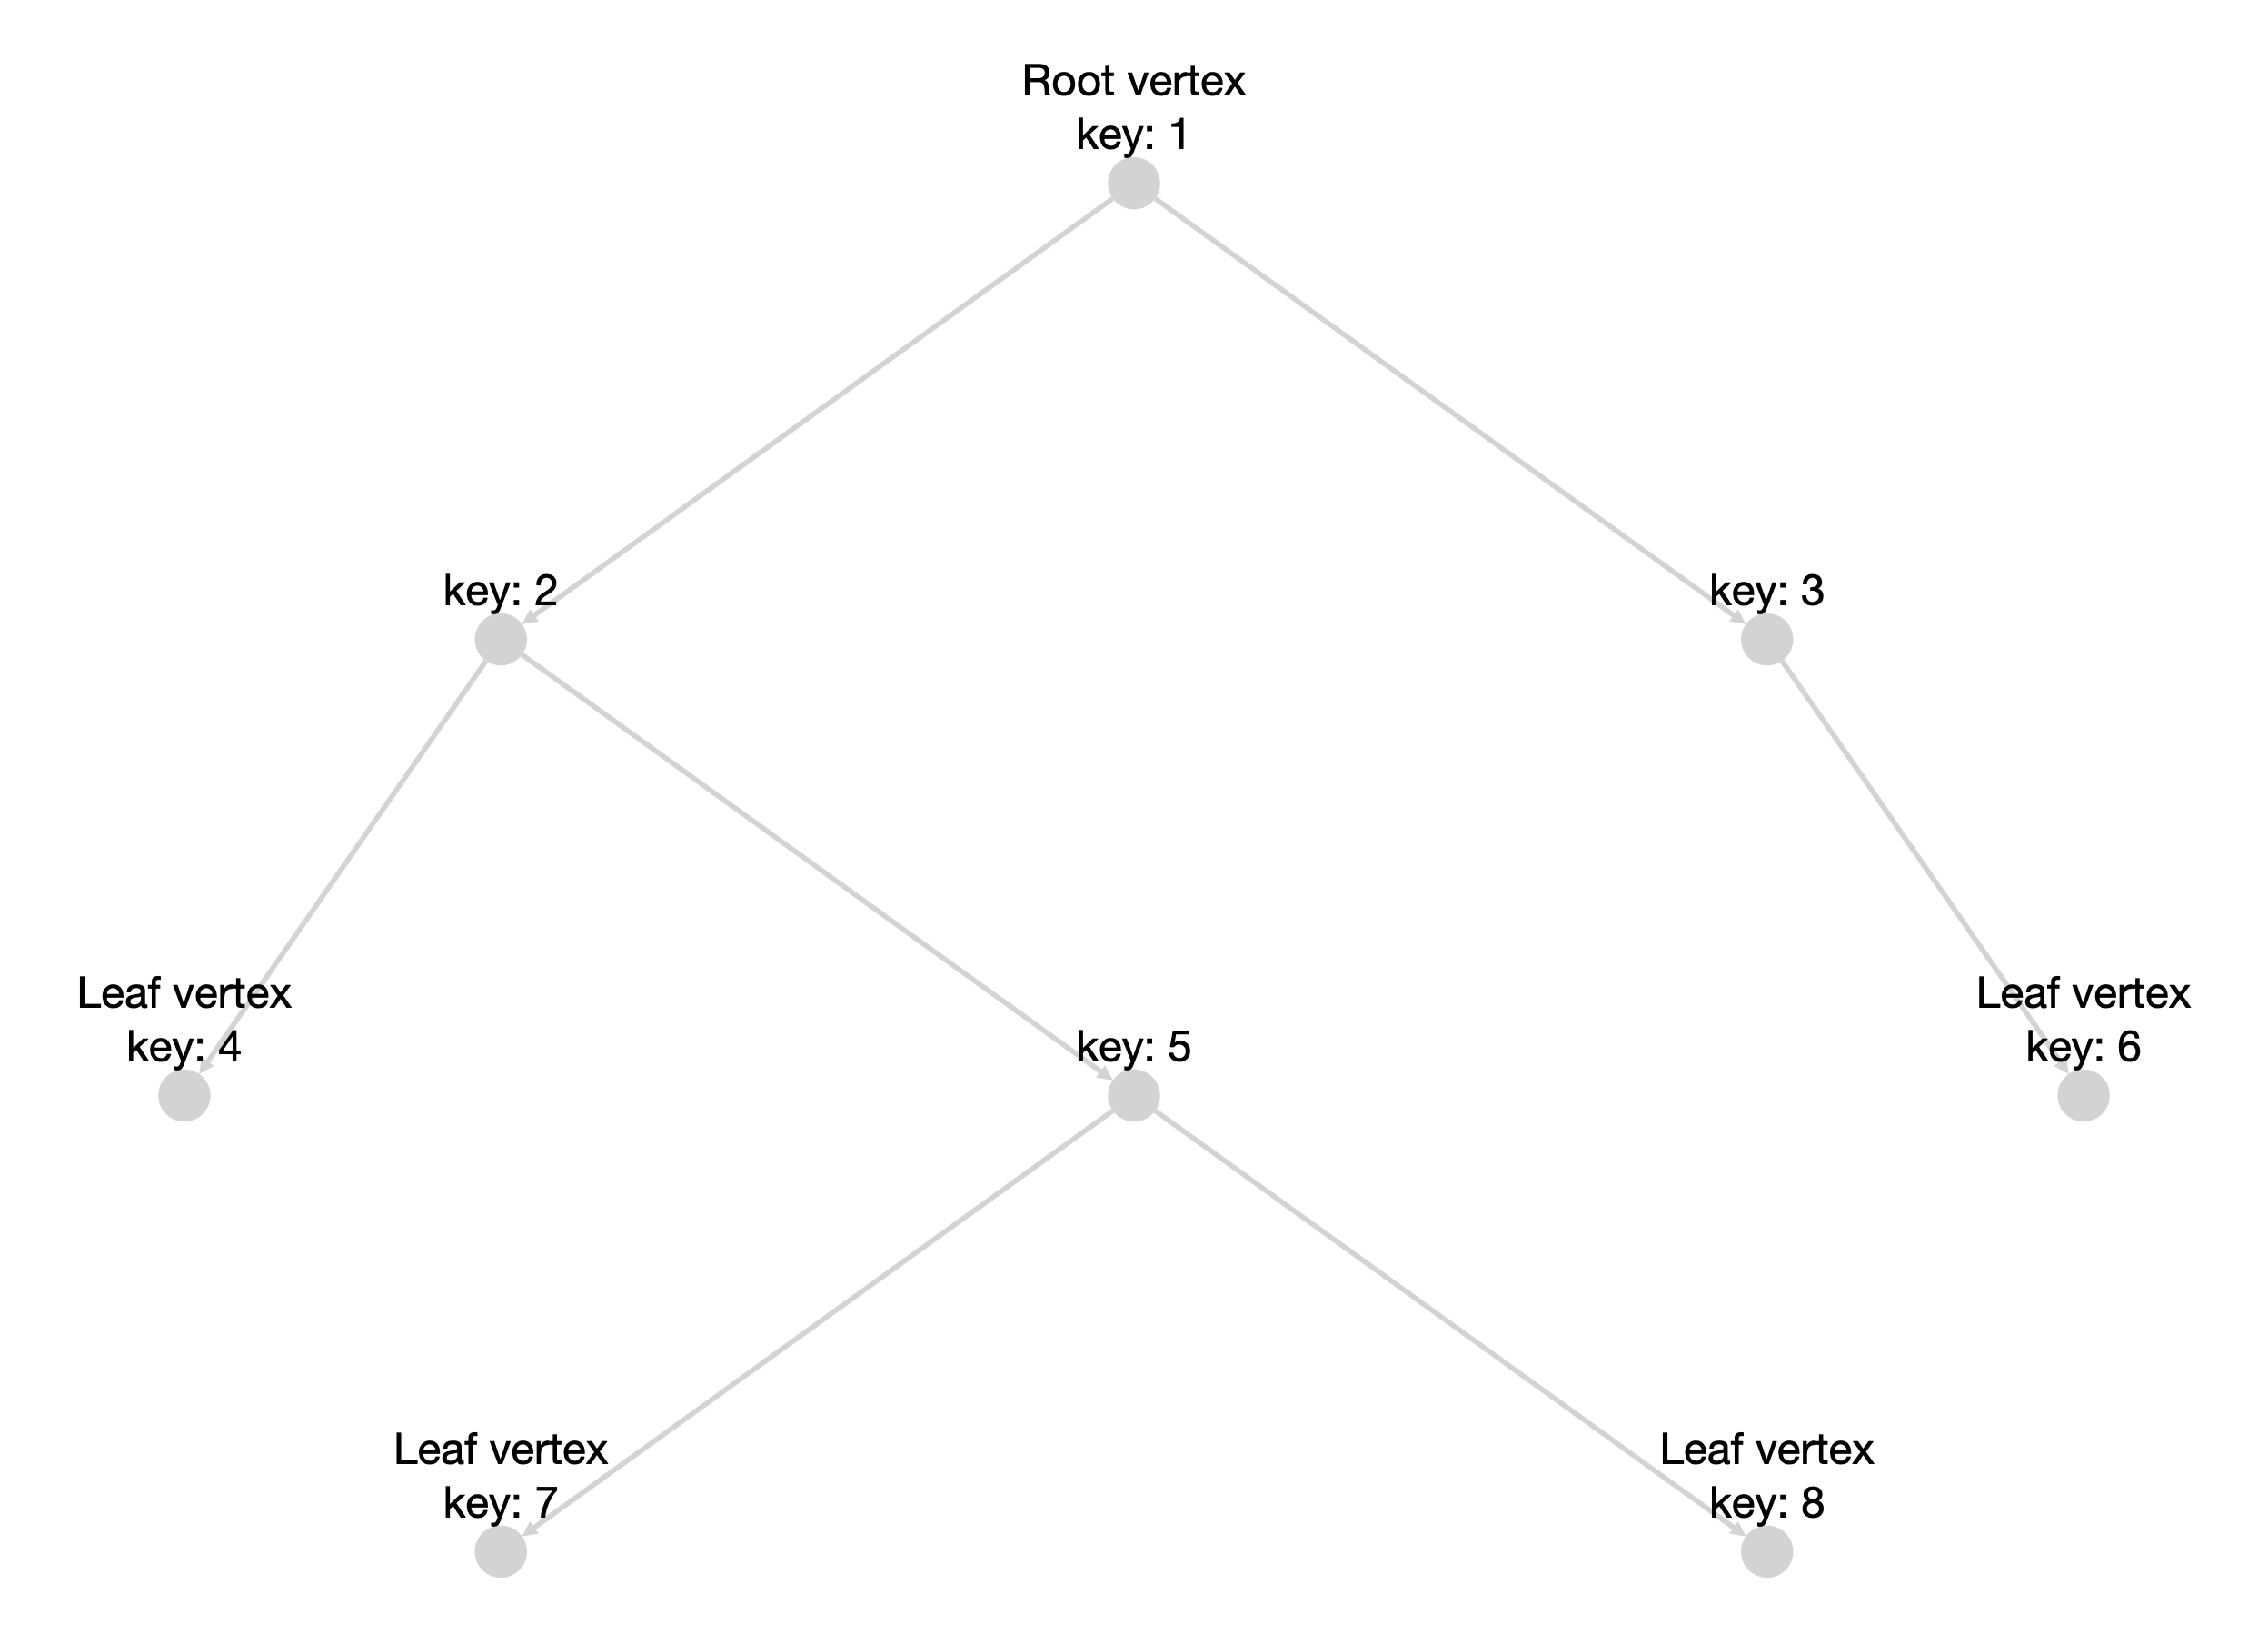
\includegraphics[scale=.175]{ps0_assets/p0_q1_BT_before.png}

 A \texttt{BinaryTree} \treeT\  contains only a pointer to its root vertex, \texttt{T.root}, which is required to satisfy \texttt{T.root.parent==None}. In the above example, 
 the root is the vertex with key 1 (i.e. \texttt{T.root.key==1}).
 A binary tree vertex \btv\ can have zero, one, or two children, determined by which of \texttt{v.left} and  \texttt{v.right} are equal to \texttt{None}.    In the above example, the vertex \btv\ with key 3 has 
 \texttt{v.left==None} but \texttt{v.right} is the vertex with key 6.
 A {\em leaf} is a vertex with zero children, i.e. \texttt{v.left==v.right==None}. 
 
 A vertex \btw\ is {\em descendent} of a vertex \texttt{v} if there is a sequence of vertices $\btv_0,\btv_1,\ldots,\btv_k$, $k\in \mathbb{N}$ such that $\btv_0=\btv$, $\btv_k=\btw$, and 
 $\btv_i \in \{\btv_{i-1}.\texttt{left},\btv_{i-1}.\texttt{right}\}$ for $i=1,\ldots,k$.\footnote{$\mathbb{N}$ denotes the natural numbers $\{0,1,2,3,\ldots\}$.  Since we are computer scientists, we start counting at 0.}
 In the above example, the vertex with key 5 is a descendent of the root (with a path of length 2), but is not a descendent of the vertex with key 3.
 The sequence $\btv_0,\btv_1,\ldots,\btv_k$ is called a {\em path} from \btv\ to \btw\ and $k$ is the {\em distance} from \btv\ to \btw. Taking $k=0$, we see that \btv\ is a descendent of itself.

 The {\em vertex set} of a binary tree \treeT\ consists of all of the descendents of \texttt{T.root}. The {\em size} of \treeT\ is its number of vertices. The {\em height} of \treeT\ is the largest distance from the root to a leaf.  The above example has size 8 and height 3.
 
 Given any vertex \btv\ in a tree, the {\em subtree} rooted at \btv\ consists of all of \btv's descendents.  Note that we can remove a subtree and turn it into a new tree \texttt{S} by setting
 \texttt{S.root=v} and \texttt{v.parent=None}.

 For now, the \texttt{key} attribute serves to distinguish vertices from each other in our tests and help illustrate what the algorithms are doing.  The \texttt{BTvertex}\ class
 also has a \texttt{size} attribute, which is initialized to \texttt{None} in all of the test instances; it will be filled in by the program you write in Part~\ref{part:calculatesizes}.

 An instance \treeT\ \texttt{BinaryTree} is {\em valid} if it satisfies the following constraints: \begin{itemize}
     \item \texttt{T.root.parent==None}
     \item \treeT\ has finitely many vertices.
     \item No two vertices \btv, \btw\ of \treeT\ share a child, i.e. 
     $\{\texttt{v.left},\texttt{v.right}\} \cap \{\texttt{w.left},\texttt{w.right}\} = \emptyset$. 
 \end{itemize}
 All of the test instances we provide are valid, and furthermore have the property that all of the vertices have distinct keys (which is something we often want, but not always).

 \begin{enumerate}
 \item \label{part:calculatesizes} (recursive programming)
 Write a recursive program \texttt{calculate\_sizes} that given a vertex \btv\ of a binary tree \treeT, calculates the sizes of all of the subtrees rooted at descendents of \btv.  After running your program on \texttt{T.root}, every vertex \btv\ in \treeT\ should have \texttt{v.size} set to the size of the subtree rooted at \btv. (Recall that the size attributes are initialized to \texttt{None}.)  We call the resulting tree a {\em size-augmented} tree.
 
For example, if \treeT\  is the  tree shown above, 
then calling \texttt{calculate\_sizes(T.root)} should modify  \treeT\ to be the following size-augmented tree:

 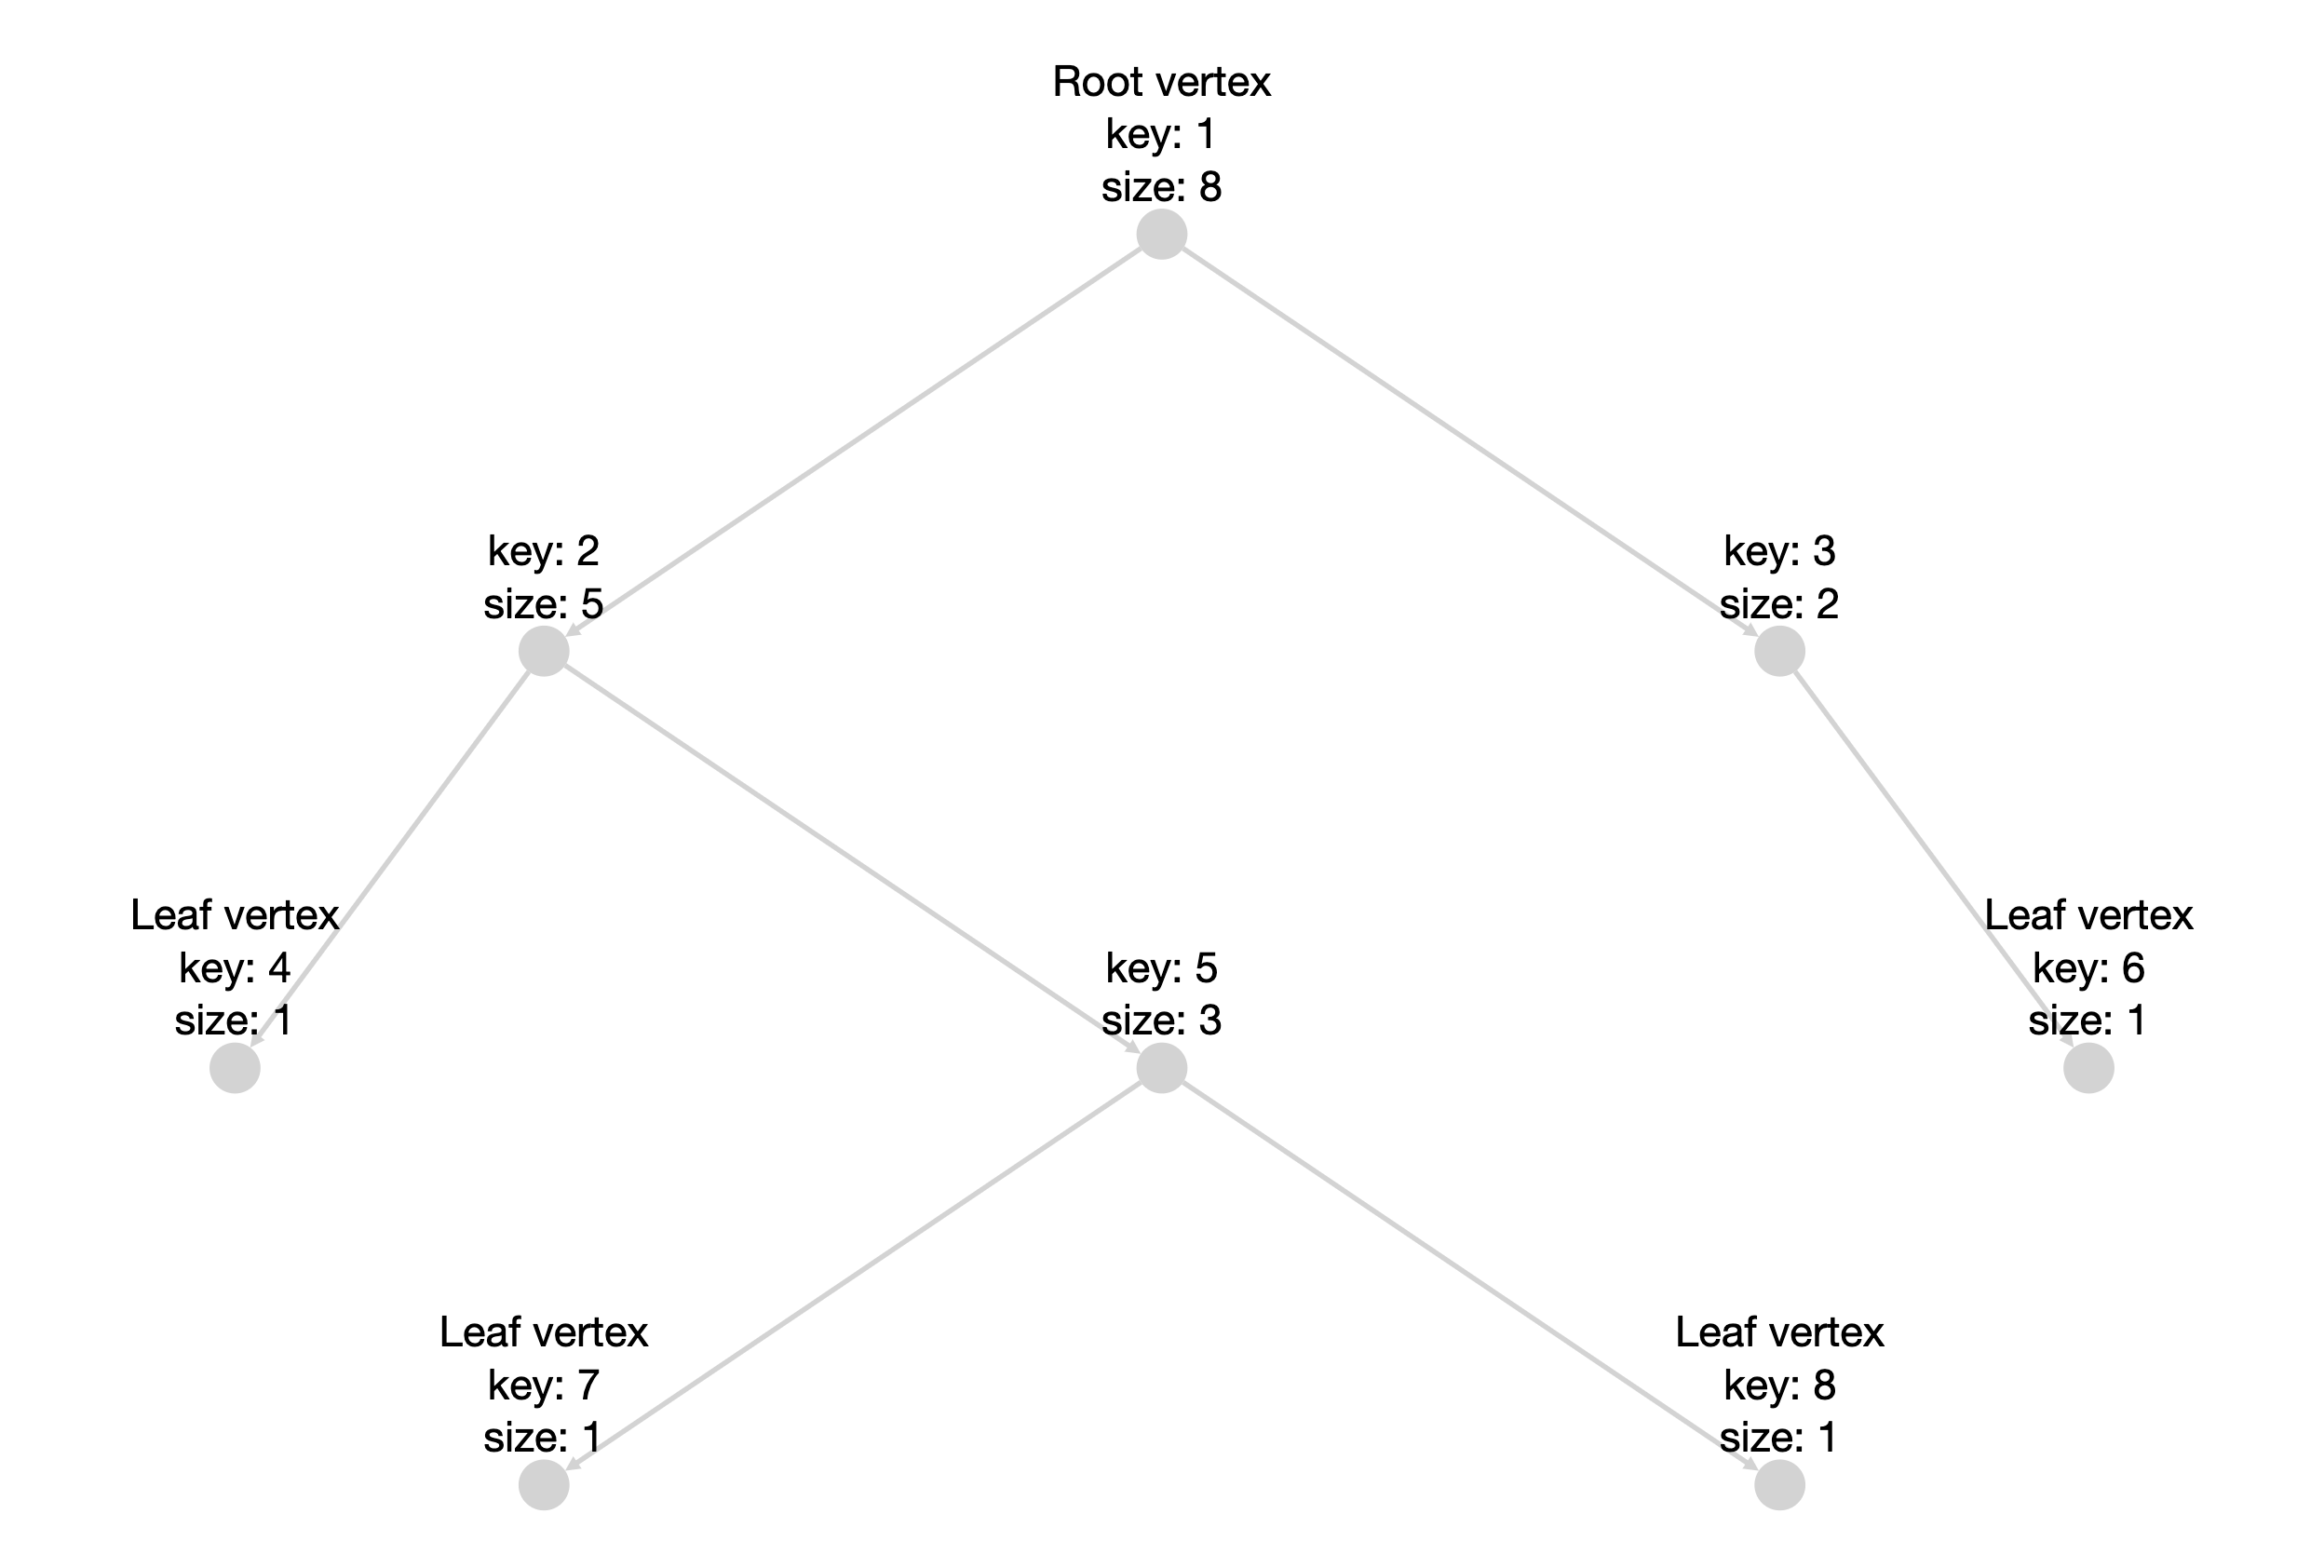
\includegraphics[scale=.175]{ps0_assets/p0_q1_BT_after.png}

 Your program should run in time $O(n)$ when given the root of a tree with $n$ vertices. In a sentence or two, informally justify why your program has such a runtime. 
 
 \item (proof warmup) \label{part:warmup}
 Removing a vertex \btv\ from a tree \treeT\ yields up to three disjoint trees: the subtree rooted at
 \texttt{v.left} (unless \texttt{v.left==None}), the subtree rooted at
 \texttt{v.right} (unless \texttt{v.right==None}), and a tree rooted at \texttt{T.root} consisting of all non-descendants of \btv\ (unless \texttt{T.root==v}).  For example:
 \\

 Before:
 
 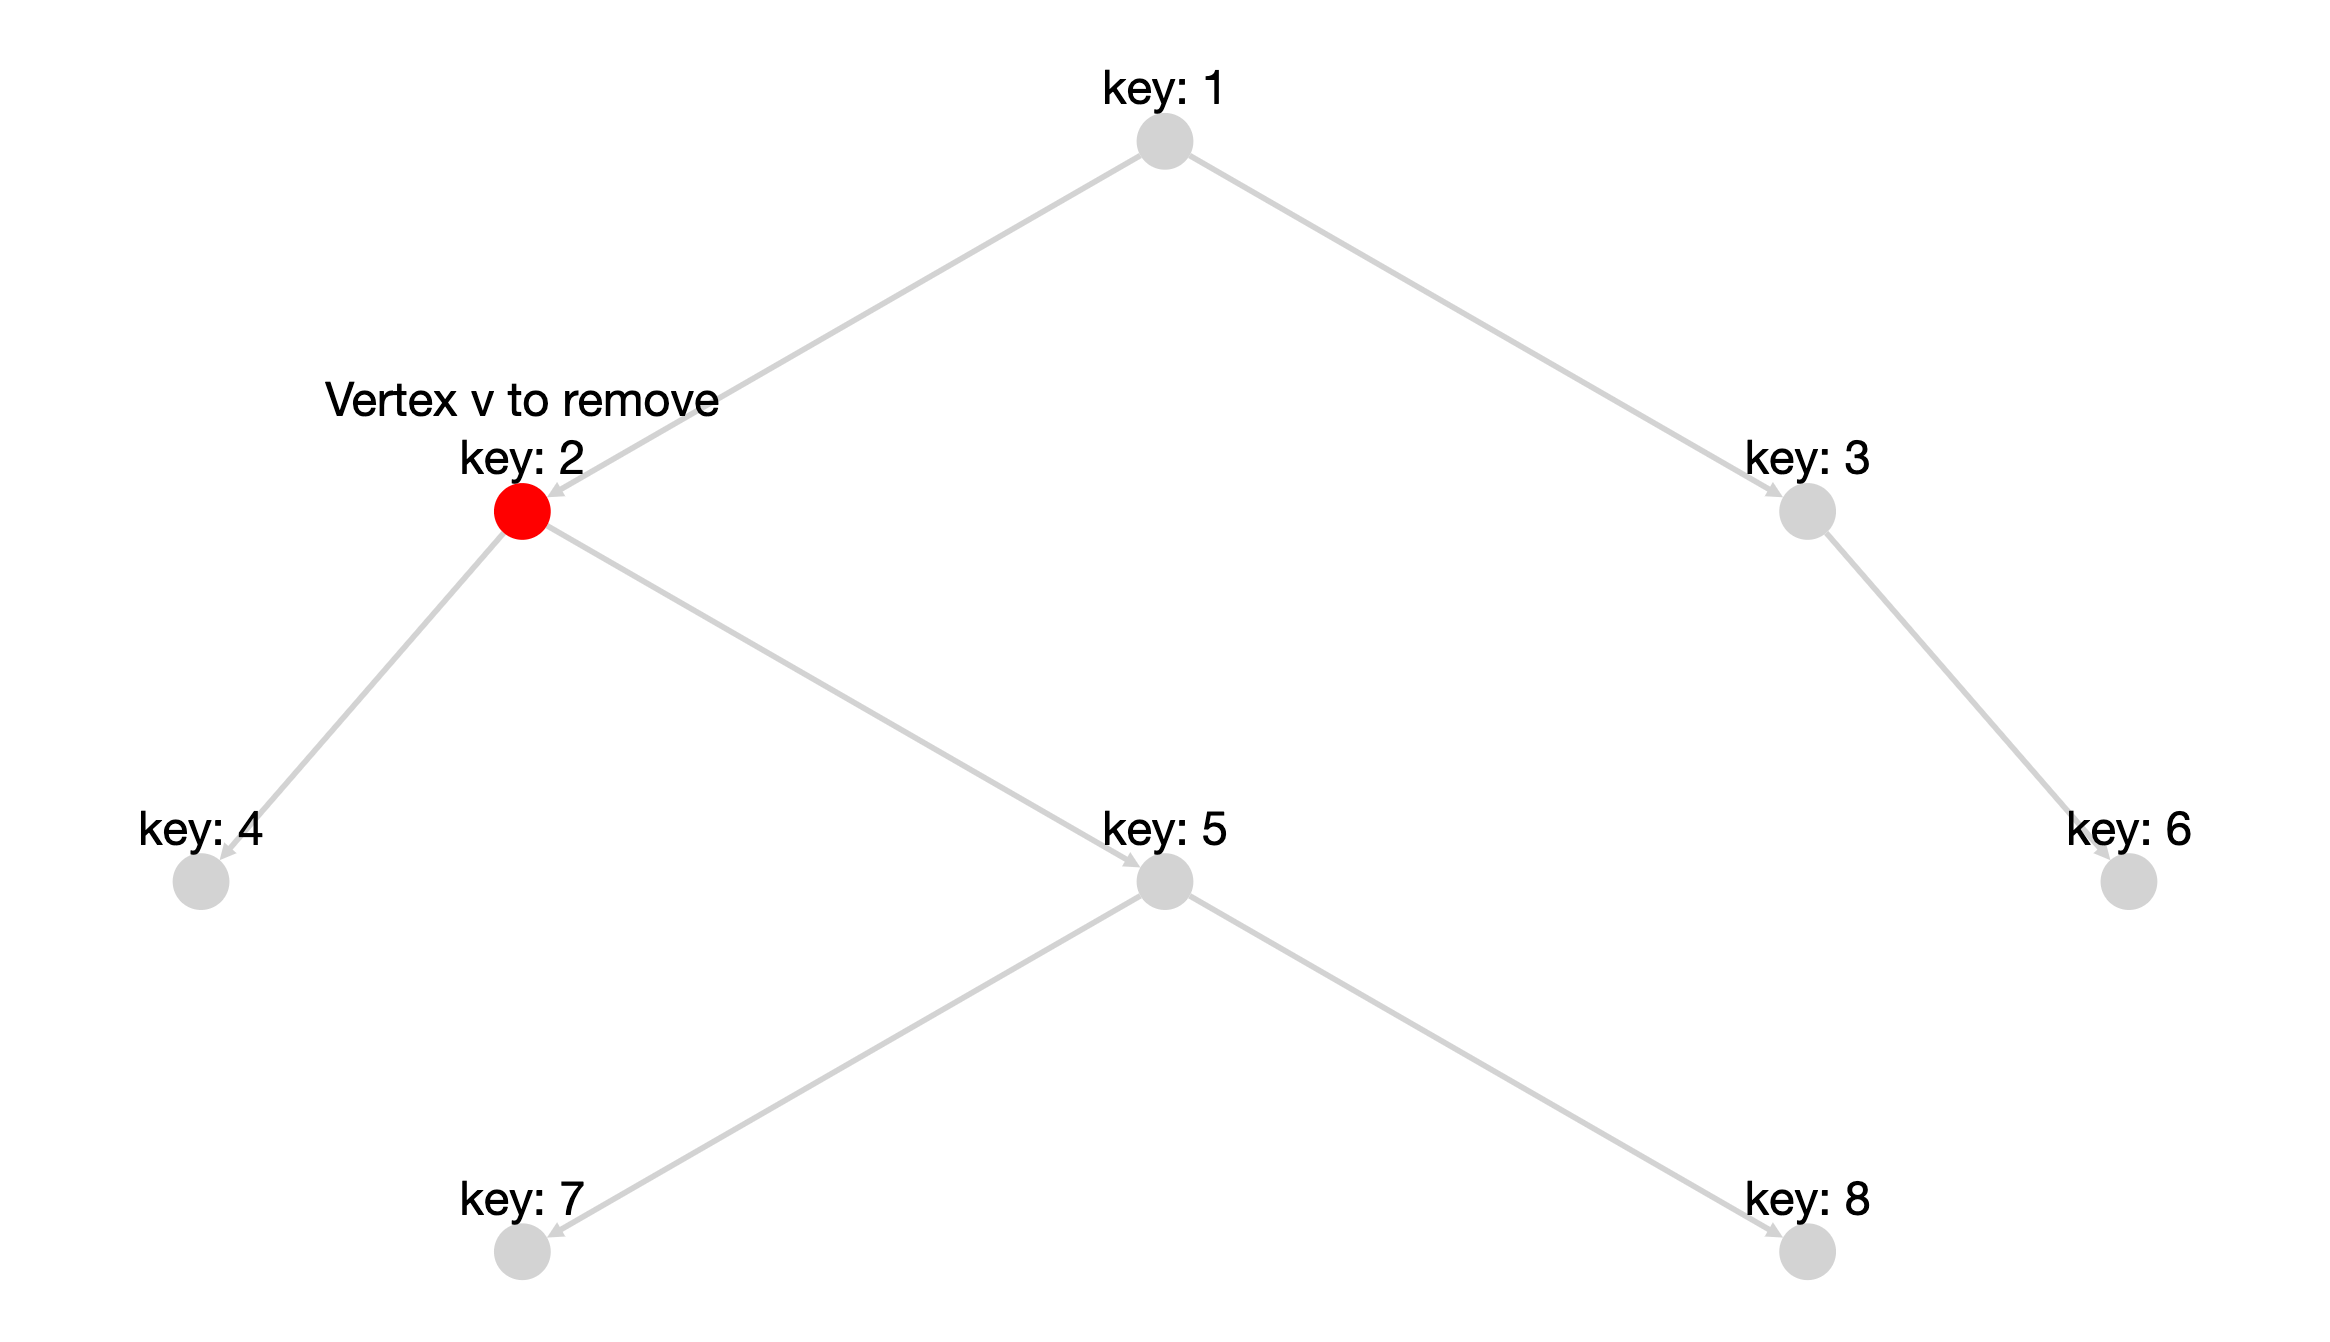
\includegraphics[scale=.175]{ps0_assets/p0_q1b_before.png}
 
 
 After:
 
  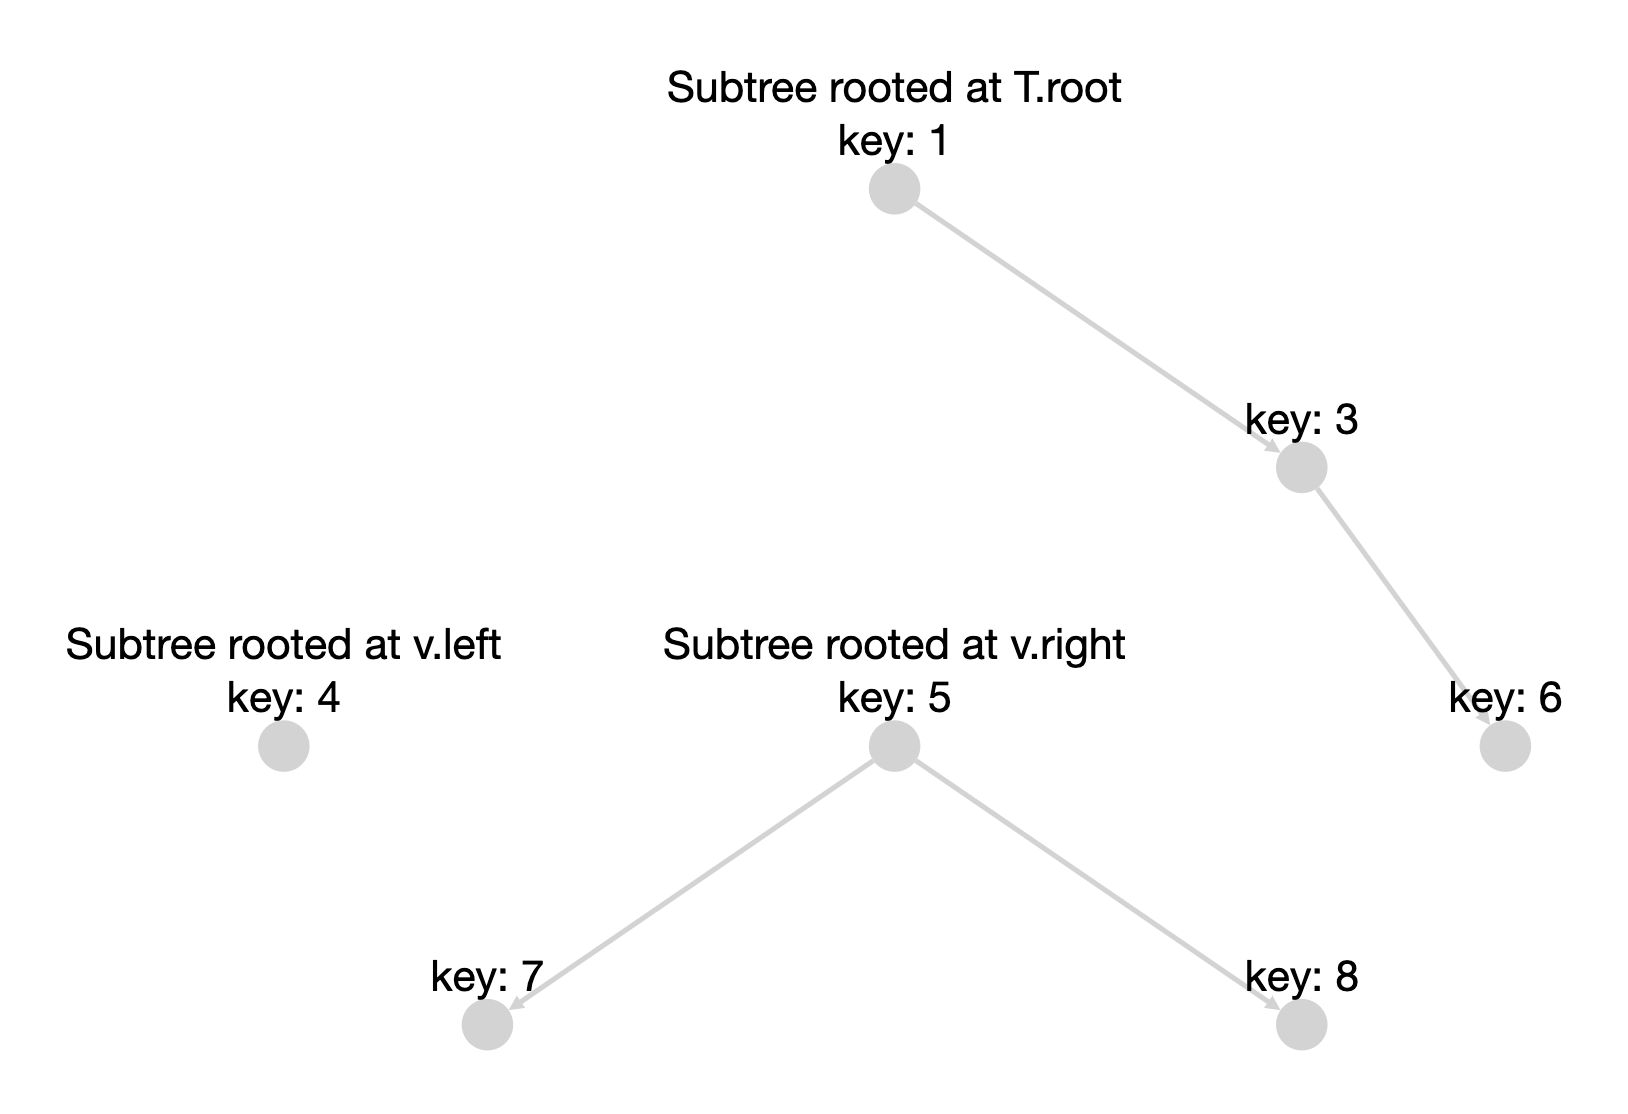
\includegraphics[scale=.225]{ps0_assets/p0_q1b_after.png}

  Suppose that for a vertex \btv, the largest subtree created by removing \btv\ contains a neighbor (i.e. child or parent) \btv$^*$\ of \btv\ and a total of $\phi(\btv)$ vertices (including \btv$^*$).
  If we remove \btv$^*$ and not \btv, we create at most two subtrees which don't contain \btv: prove that these subtrees each contain fewer than $\phi(\btv)$ vertices.

 \item (proofs by contradiction) \label{part:contradiction}
  Prove that in every tree \treeT\ of size $n$, there exists a vertex \btv\ such that removing \btv\ from \treeT\ results in disjoint trees that all have size at most $n/2$.  \\

  You may prove this however you like, but a recommended approach is to extend Part~\ref{part:warmup} and show that if the largest subtree created by removing a vertex \btv\ contains a neighbor \btv$^*$ of \btv\ and contains $\phi(\btv) > n/2$ vertices, then if we remove \btv$^*$ and not \btv, the subtree \emph{containing} \btv\ contains at most $n/2$ vertices. Then choose \btv\ to be the vertex for which $\phi(\btv)$, the size of the largest tree created by removing \btv, is smallest.

 \item (from proofs to algorithms)  Turn your proof from Part~\ref{part:contradiction} into a Python program that given a root vertex \texttt{r} of a {\em size-augmented} tree \treeT\ with $n$ vertices finds a vertex \btv\ with $\phi(\btv)\leq n/2$. Your program should run in time $O(h)$ on all size-augmented trees of height $h$; again informally justify why your program has such a runtime. (Hint: try to repeatedly reduce the potential function by moving to children. Why don't we need to try moving to parents as in the previous proof?)
 \end{enumerate}
 
 \newcommand{\incomp}{\mathit{incomp}}
 \item (matchings and induction)
 Later in the course, we will study matching algorithms that are used in practice to match kidney donors to patients.  The challenge in general is that some donors are incompatible with some patients (i.e. the patient's body is likely to reject the donated kidney).  Suppose we are very lucky and have $n$ donors and $n$ patients where each donor $d$ is incompatible with exactly one patient, denoted $\incomp(d)$, and each patient $p$ is incompatible with exactly one donor $\incomp(p)$. (Incompatibility is symmetric, so $\incomp(d)=p$ iff $\incomp(p)=d$.)  Let $f(n)$ be the number of ways, under these circumstances, of matching donors to patients so that each donor donates exactly one kidney to a compatible patient and each patient receives exactly one kidney from a compatible donor.  


 \begin{enumerate} 
\item Show that for all $n\geq 3$,
 $$ f(n) > (n-1)\cdot f(n-2).$$
 Hint: let $d$ be one of the donors, and consider all possible patients $p$ with whom $d$ could be matched.  Then consider the case where $\incomp(p)$ is matched with $\incomp(d)$.

 \item
 In fact, show that for all $n\geq 3$, we have
 $$ f(n) = (n-1)\cdot (f(n-1)+f(n-2)).$$
 This will require you to include the remaining case where $\incomp(p)$ is \emph{not} matched with $\incomp(d)$, unlike the previous exercise.

 \item 
 Prove by strong induction that for all $n\geq 2$,
 $$\frac{n!}{3} \leq f(n) \leq \frac{n!}{2}.$$
 \end{enumerate}



\end{enumerate}


\end{document}
